\section{Ejercicio 8}

Presentamos el siguiente lote corrido con distintos semillas de aleatoridad y tamaño de quantum.

Fijar semilla

TaskBatch 10 1 \\
TaskBatch 10 1 \\
TaskBatch 11 3 \\
TaskBatch 10 4 \\
TaskBatch 10 3 \\
TaskBatch 10 2 \\


Se elige este lote para mostrar procesos similares que asimple vista pueden llegar terminar juntos bajo un scheduler DETERMINISTICO pero la aleatoridad será un punto clave ya que al ser un factor externo sin relacion con los procesos hará que a los procesos se le asignen de diferentes maneras a partir de su compartamiento en cada corrida. 


quantum por vez, para ver como el buen compartmiento afecta la aleatoridad
2,5,9,12,15
\begin {center}
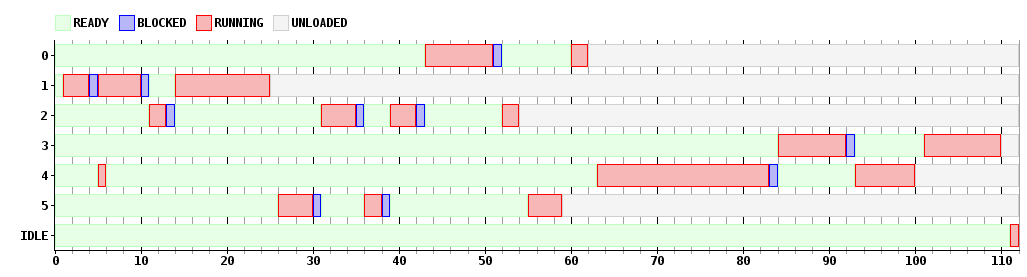
\includegraphics[width=16cm]{../simusched/outputs/loterya.png}
\end {center}
\begin {center}
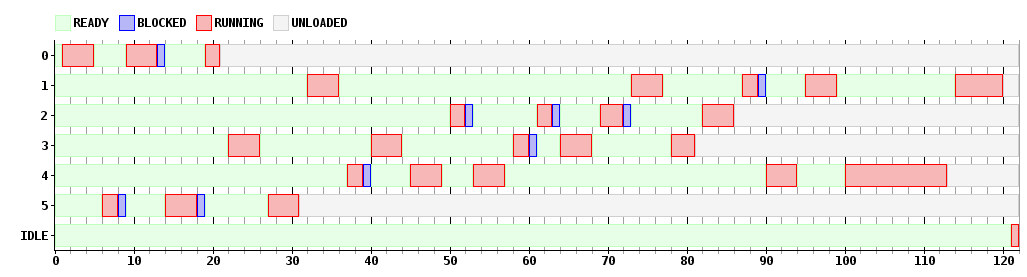
\includegraphics[width=16cm]{../simusched/outputs/loteryc.png}
\end {center}
\begin {center}
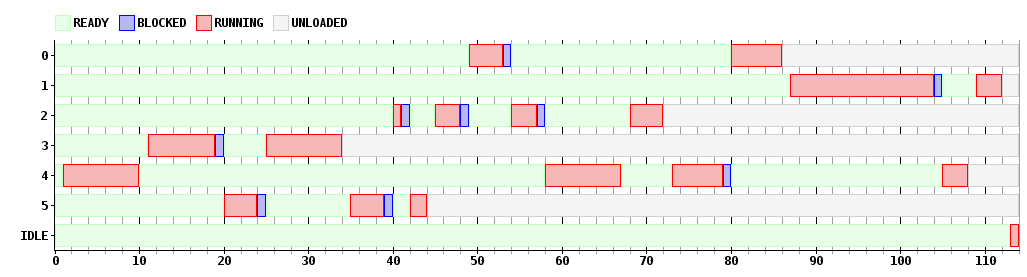
\includegraphics[width=16cm]{../simusched/outputs/loteryd.png}
\end {center}
\begin {center}
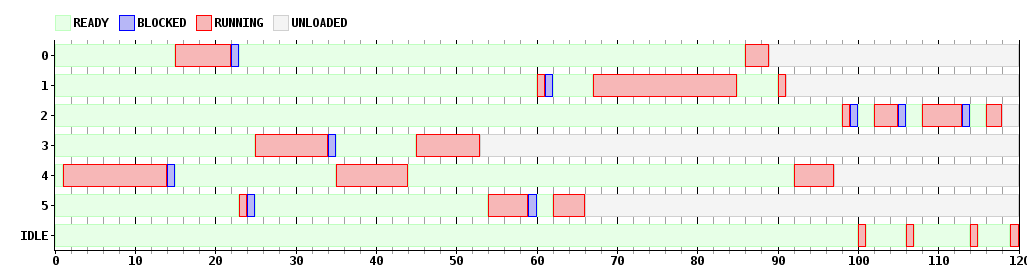
\includegraphics[width=16cm]{../simusched/outputs/loterye.png}
\end {center}
\begin {center}
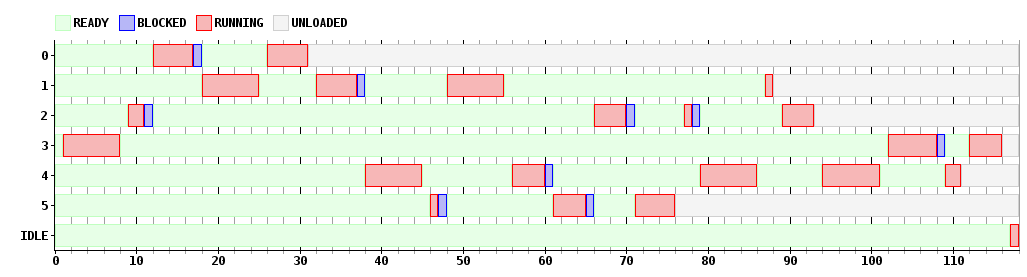
\includegraphics[width=16cm]{../simusched/outputs/loteryf.png}
\end {center}



Se puede notar que aunque se elija el mismo lote, la aleatoridad del algoritmo muestra como aunque se asignen de distinta forma los recursos, todos los procesos
tienden a obtenerlos uniformemente.\\

Cuenta tiempo de espera para cada gantt y ver que son parecido, si no son parecidos, cambiar linea ed arriba


Utilizamos el mismo ejemplo para notar la $"$compensación$"$. Notese como en el A el proceso 1 después de haber bloqueado 2 veces obtuvo tantos tickets que casi tuvo
exclusividad del procesador. Por el contrario el proceso 4 tuvo que esperar varios sorteos hasta salir ganador.
